\chapter{Theoretical Framework}
\section{Sequential Decision-Making}
In robotics, sequential decision-making problems refers to tasks in which a robot must achieve a goal by physically interacting with the environment, for example, navigating from one point to another, grasping an object, balancing, etc. It can be described as a step-by-step decision theory, where depending on the information that is gathered by its sensors, the robot has to make decisions consecutively.

\subsection{Markov Decision Process (MDP)}
A Markov Decision Process (MDP) is meant to be a straightforward framing of sequential decision-making problems. In a MDP we have an \emph{agent} and an \emph{environment}, which interact continually. The agent is the learner and the decision maker. The environment is everything that the agent can interact with\cite{sutton}. In robotics, the agent is the robot and the environment is the setting, in the real world, in which the robot interacts.

To keep things as simple as possible, MDPs are commonly modeled as discrete time interaction of the agent with the environment. Thus, the time is divided into a sequence of \emph{time steps}, $t=0,1,2,3,...$ . At each time step the agent \emph{observes} \textbf{($o_{t}$)} a representation of the environment's \emph{state} \textbf{($s_{t}$)}. Depending on the state, the agent selects an \emph{action} \textbf{($a_{t}$)}, that, ideally, will lead to achieving the goal of the task.

The state describes the current situation of the environment; the action is an input to the environment that the agent can select and that affects the environment's evolution. The agent receives a representation of the state which is called the observation. In robotics, this is information gathered with sensors such as RGB cameras, encoders, inertial measurement units, etc. If the observation contains sufficient information such that the agent can fully understand the environment state, then the problem is said to be \emph{fully observed}, otherwise, is called \emph{partially observed}. If a partially observed problem is modeled with a MDP, then is called a partially observable MDP, or POMDP.

The environment's evolution is the sequence of states visited by the agent. Transitioning from one state to another is a stochastic process defined by the nature of the environment and the actions taken, at each time step, by the agent. Additionally, a MDP is formulated as an extension of a Markov chain, such that the Markov property is satisfied. As a consequence, the conditional probability distribution of future states depends only upon the present state, such that:

\begin{equation}
    \mathsf{P}(s_{t}|s_{t-1}, a_{t-1}) = \mathsf{P}(s_{t}|s_{t-1},...,s_{0},a_{t-1},...,a_{0})  \hspace{0.5cm} \forall t
\end{equation}

Finally, every time the environment transitions, a numerical \emph{reward} is received by the agent. Better decisions will produce higher rewards.

In a nutshell, a MDP can by defined by the tuple $MDP=(\mathcal{S},\matchcal{A},\mathcal{R},\mathcal{P})$, where $\mathcal{S}$ represents the state space and $\mathcal{A}$ the action space. $\mathcal{R}$ represents the \emph{reward function}, which generates a scalar reward every time step. This reward may depend on $s_{t-1}$; $s_{t-1},a_{t-1}$ or $s_{t-1},a_{t-1},s_{t}$, so $\mathcal{R}$ can be defined with $\mathcal{R}: \mathcal{S} \to \R$, $\mathcal{R}: \mathcal{S} \times \mathcal{A} \to \R$ or $\mathcal{R}: \mathcal{S} \times \mathcal{A} \times \mathcal{S} \to \R$, respectively. Finally, $\mathcal{P}$ corresponds to the transition function, which is the probability $\mathsf{P}(s_{t+1}|s_{t}, a_{t})$, where $\mathcal{P}: \mathcal{S} \times \mathcal{A} \times \mathcal{S} \to [0, 1]$. Graphically, a MDP can be summarized in the following diagram:

\begin{figure}[H]
    \centering
    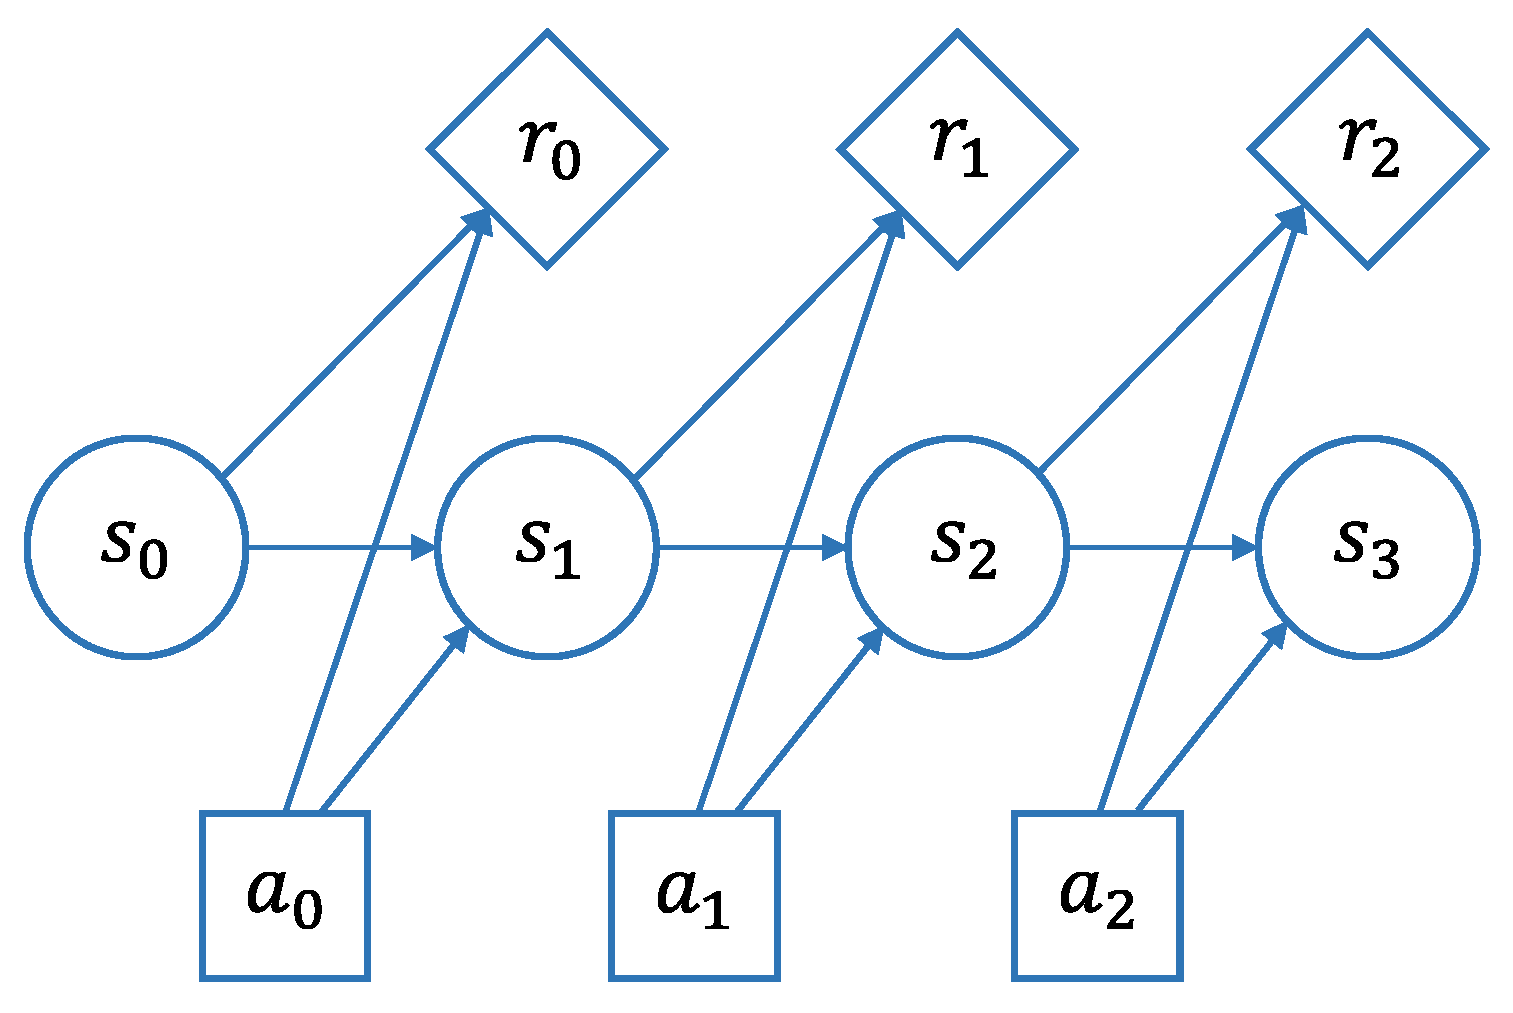
\includegraphics[width=0.7\linewidth]{imagenes/cap1/mdp.png}
    \caption{Finite part of a Markov Decision Process.}
    \label{fig:msim}
\end{figure}

\subsection{Reinforcement Learning}
Reinforcement Learning aims to use the MDP framing of sequential decision-making problems so that agents learn to solve tasks from \emph{experience}. In this case, experience is understood as the agent-environment interaction, which results in the generation of reward values that indicates the quality of the decisions made by the agent. The idea is to, somehow, use this experience to \textbf{maximize the expected return}. The return \textbf{($G$)} is simply the sum of the rewards \textbf{($r$)}:

\begin{equation}
G_{t} = \sum_{i=t+1}^{T}r_{i}
\end{equation}


\subsubsection{Value Function Approximation}
\subsubsection{Policy Gradient}
\subsubsection{On/Off Policy}
\subsubsection{Replay Buffer}


\subsection{Function Approximation}
\subsubsection{Linear Model of Basis Functions}
\subsubsection{Artificial Neural Networks}
\subsubsection{Feedforward Fully-Connected}
\subsubsection{Convolutional}
\subsubsection{Autoencoder}
\subsubsection{Recurrent}
Long Short-Term Memory

\subsection{Learning from Demonstration}
\subsubsection{The Correspondence Problem}
\subsubsection{Distributional Drift}
\subsection{Learning from Feedback}
\subsubsection{Evaluative Feedback}
\subsubsection{Corrective Feedback}
When teaching with human corrective advice, if the agent executes an action $a$ that the human considers to be erroneous, then s/he would indicate the direction in which the action should be corrected (thus, COACH was proposed for problems with continuous actions). Each dimension of the action would have a corresponding correction signal $h$ with values $0$, $-1$ or $1$ which produces an error signal with arbitrary magnitude $e$ that is used to shape directly the policy. Thus, the error would be: 
\begin{equation}\label{eq:error}
    error=h \cdot e.
\end{equation}

$h=0$ indicates that no correction has been advised. $h=\pm 1$ indicates the direction of the advised correction.

\section{COrrective Advice Communicated by Humans (COACH)}
In this framework no value function is modeled, since no reward/cost is used in the learning process \cite{Celemin2018AnInteractive}. A parametrized policy is directly learned in the parameter space, as in Policy Search (PS) RL. 
The classic COACH algorithm shapes two functions parametrized as a linear model of basis functions. The objective of the first function is to learn the policy of the agent $\pi(s)=f^{\top}\theta$; the objective of the second function, $H(s)=f^{\top}\psi$, is to learn a prediction of the human feedback. The vector of basis functions $f(s)$, for simplicity is called $f$. The parameter vectors $\theta$ and $\psi$ are updated to shape the models. As it can be seen, $f$ is the same vector for both the Policy Model $\pi(s)$ and the Human Feedback Model  $H(s)$. The Human Feedback Model is used to adapt the size of the error signal that is then used to update the weights of $\pi(s)$. Both functions are updated using stochastic gradient descent each time feedback is received. The pseudocode of COACH is shown in Algorithm \ref{algorithm:COACH}.

\begin{algorithm}[H]
\caption{Basic Structure of COACH}\label{algorithm:COACH}
\begin{algorithmic}[1]
\State \textbf{Require:} error magnitude $e$, human model learning rate $\beta$, time steps $N$
\For{t = 1,2,...,N}{}
\State \textbf{observe} state $s_{t}$
\State \textbf{execute} action $a_{t}=\pi(s_{t})$
\State \textbf{feedback} human corrective advice $h_{t}$
\If{$h_{t}$ != 0}
\State \textbf{update} $H(s_{t})$ with $\Delta \psi = \beta\cdot (h_{t}-H(s_{t}))\cdot f$
\State $\alpha_{t} = |H(s_{t+1})|$
\State $error_{t} = h_{t}\cdot e$
\State \textbf{update} $\pi(s_{t})$ with $\Delta \theta = \alpha_{t} \cdot error_{t} \cdot f$
\EndIf
\EndFor
\end{algorithmic}
\end{algorithm}